\chapter{Functions of several variables.} 

\section{$n$-dimensional space}    %{{{1
The line is one-dimensional, the plane is two dimensional, and the
space around us is three dimensional\footnote{Although some physicists
will tell you it's really 11 or 24 dimensional.}.

A point on the line is specified by one coordinate ``$x$'', a point in
the plane by two coordinates, ``$(x, y)$'', and a point in three
dimensional space can be specified by three coordinates $(x, y, z)$.
Going on like that, a point in $56$-dimensional space is specified by
$56$ coordinates, $(x_1, x_2, \dots, x_{55}, x_{56})$.
Instead of getting philosophical about what $n$-dimensional space
really is (``does it exist?''), we simply say that a point in
$n$-dimensional  space is a list of $n$-real numbers, $(x_1, \dots,
x_n)$ and that, as far as mathematics is concerned, $n$-dimensional
space is just the collection of all possible lists $(x_1, \cdots,
x_n)$ of $n$ numbers.  If $n=1, 2$, or $3$, then we can visualize such
a point by drawing one, two or three axes;  if $n=4$ or more, then we
can't, but it doesn't matter.

The symbol $\R^n$ is used to stand for $n$-dimensional space, meaning
the collection of all such lists of $n$ numbers $(x_1, \dots, x_n)$.

In this course we will mostly deal with $\R^2$ and $\R^3$, although
much of what we do works (and gets used) without modification in $\R^n$.


\section{Functions of two or more variables}    %{{{1

\subsection{The graph of a function}    %{{{2
In first-year calculus we were concerned with functions of one
variable, meaning the ``input'' is a single real number and the
``output'' is likewise a single real number. At the end of math 222 we
considered functions taking a real number to a vector: for each input
value we get a position in space. Now we turn to functions of several
variables, meaning several input variables, functions.
While we will deal primarily with $n=2$ and to a lesser
extent $n=3$, many of the techniques we discuss can be applied
to larger values of $n$ as well. 

\begin{figure}[h]
  \begin{center}
    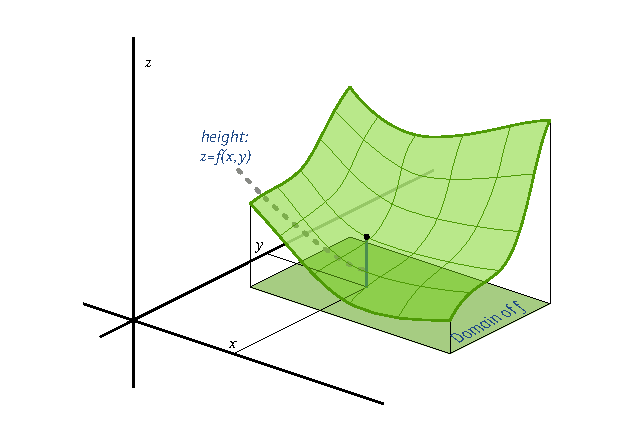
\includegraphics{01Agraph.pdf}
  \end{center}
  \caption{The graph of some function, and its domain (a rectangle in
  this example).}
  \label{fig:01Agraph}
\end{figure}

A function of two variables maps a pair of values $(x,y)$ to a
single real number.  The three-dimensional $xyz$-coordinate system 
is a convenient aid in visualizing such functions: above
each point $(x,y)$ in the $xy$-plane we graph the point $(x,y,z)$,
where of course $z=f(x,y)$. 

\subsection{Vector notation} We will use vectors all the time in this    %{{{2
course.  If $\vx$ is the position vector of the point $(x, y)$ in the
plane, i.e.\ if $\vx = \tvek x\\ y\ttor$, then one writes
\[
f(x, y)  = f(\vx).
\]

\subsection{Example}\label{sec:example-of-a-function1} Consider    %{{{2
$f(x,y)=3x+4y-5$. Writing this as $z=3x+4y-5$ and then $3x+4y-z=5$ we
recognize the equation of a plane.  In the form $f(x,y)=3x+4y-5$ the
emphasis has shifted: we now think of $x$ and $y$ as independent
variables and $z$ as a variable dependent on them, but the geometry is
unchanged.

\subsection{Example}\label{sec:example-of-a-function2} You know that    %{{{2
$x^2+y^2+z^2=4$ represents a sphere of radius 2. We cannot write this
in the form $z=f(x,y)$, since for each $x$ and $y$ in the disk
$x^2+y^2<4$ there are two corresponding points on the sphere. As with
the equation of a circle, we can resolve this equation into two
functions, $f(x,y)=\sqrt{4-x^2-y^2}$ and $f(x,y)=-\sqrt{4-x^2-y^2}$,
representing the upper and lower hemispheres. Each of these is an
example of a function with a restricted domain: only certain values of
$x$ and $y$ make sense (namely, those for which $x^2+y^2\le 4$) and
the graphs of these functions are limited to a small region of the
plane.


\subsection{Freezing a variable}    %{{{2
\begin{multicols}{2}
If a function isn't familiar, then a good strategy for drawing its
graph is to ``\emph{freeze a variable.}'' In other words, to analyze
a function $ z=f(x,y) $ you pretend $ y $ is a constant: then $ x $
is the only independent variable, and you can try to draw the graph
of the function $ z=f(x,y) $, now thinking of this as a function of
only one variable. This graph is a curve in the $ xz $ plane. You
get one such curve for each choice of $ y $. Piecing these graphs
together then gives you the graph of the two-variable function $
z=f(x,y) $.

You could apply the same procedure with the roles of $ x $ and $ y $
switched: i.e. for each fixed $ x $ you try to graph $ z=f(x,y) $ as
a function of the variable $ y $ only, after which you try to fit
all the graphs you get for different values of $ x $ together.

\centerline{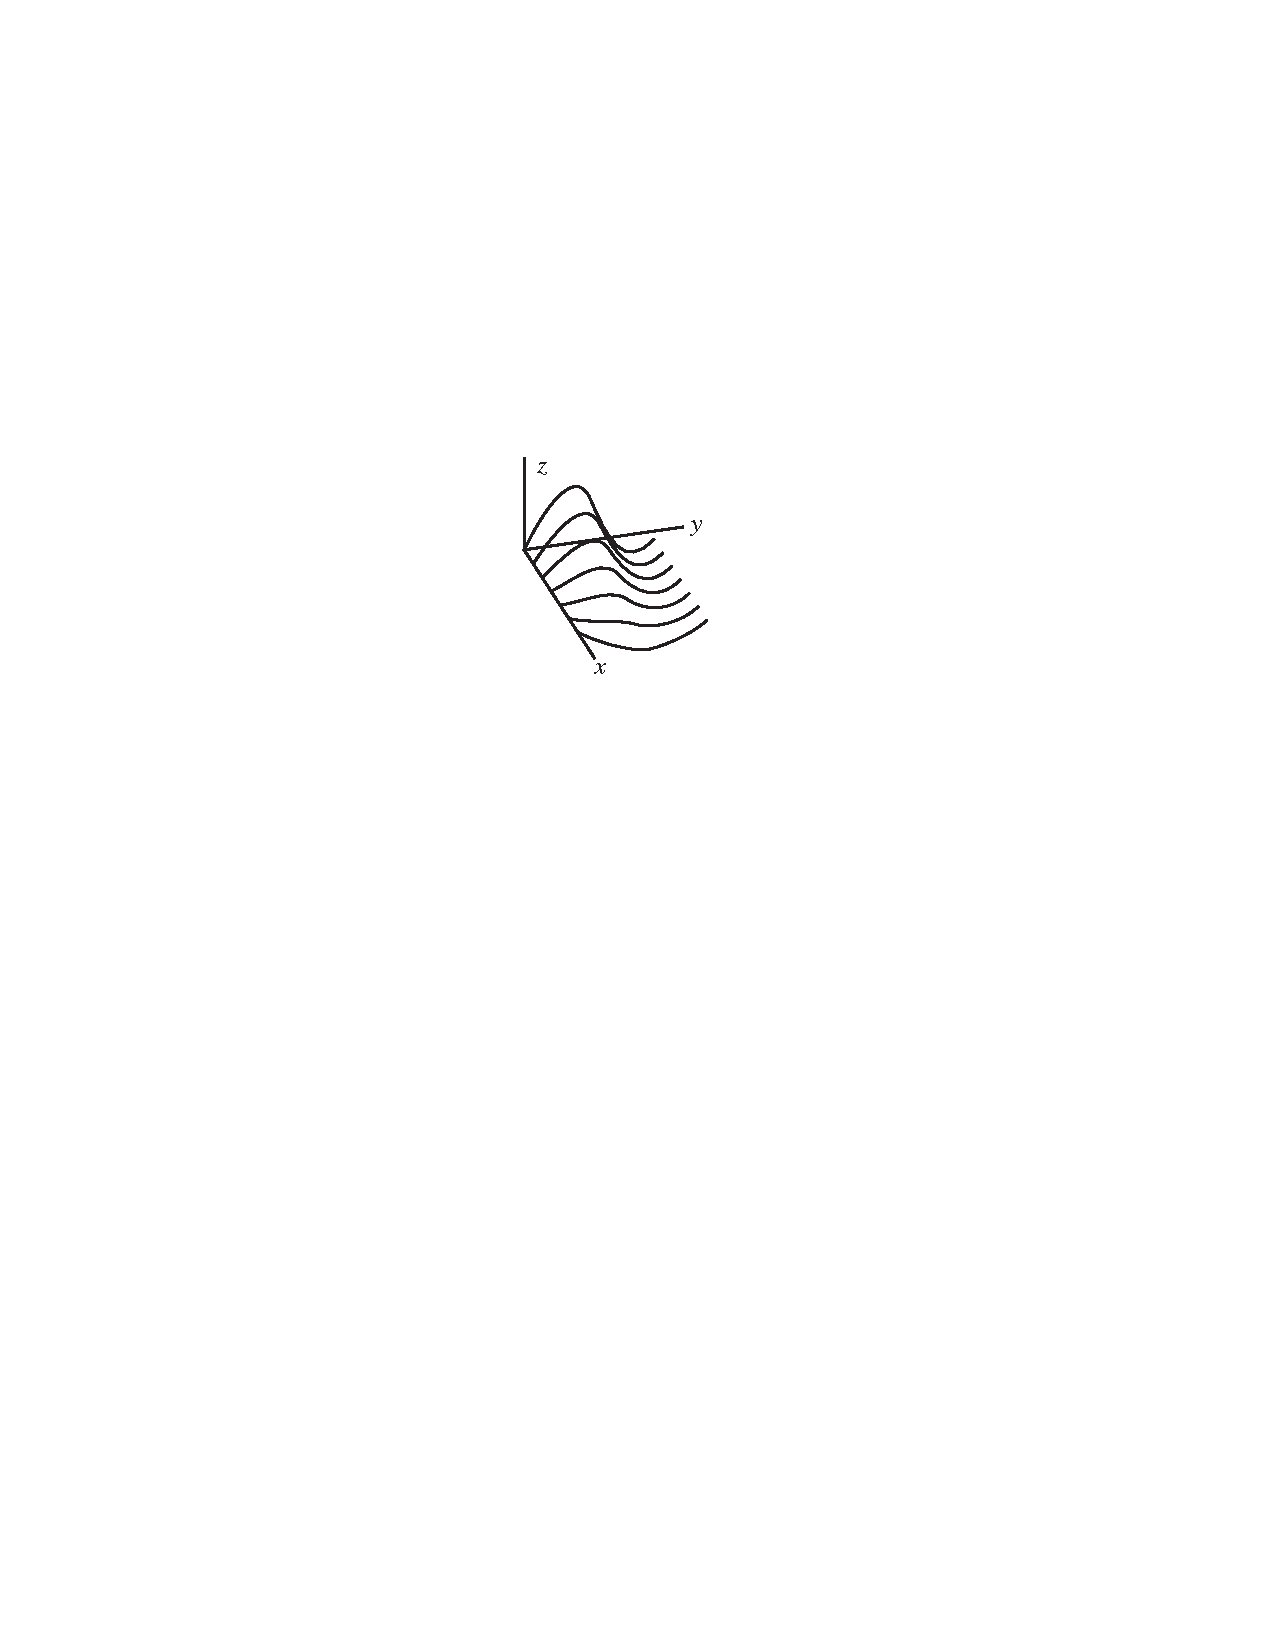
\includegraphics{01frozenvariable.pdf} }
\end{multicols}



\subsection{Example -- draw the graph of $f(x,y) = xy$}    %{{{2
\label{sec:example-of-a-function3}
Let's plot the graph of $ z=f(x,y)=xy $.  For each fixed value of $ y $
the graph of $ f(x,y)=xy $ is a straight line with slope $ y $.  For
positive $ y $ the line has positive slope, for negative $ y $ it has
negative slope.   Plotting the graphs of $ z=xy $ for $ y $ frozen at
the values -1,$ -\frac{1}{2} $, $ 0 $, $ \frac{1}{2} $, and 1 gives us
these drawings:

\centerline{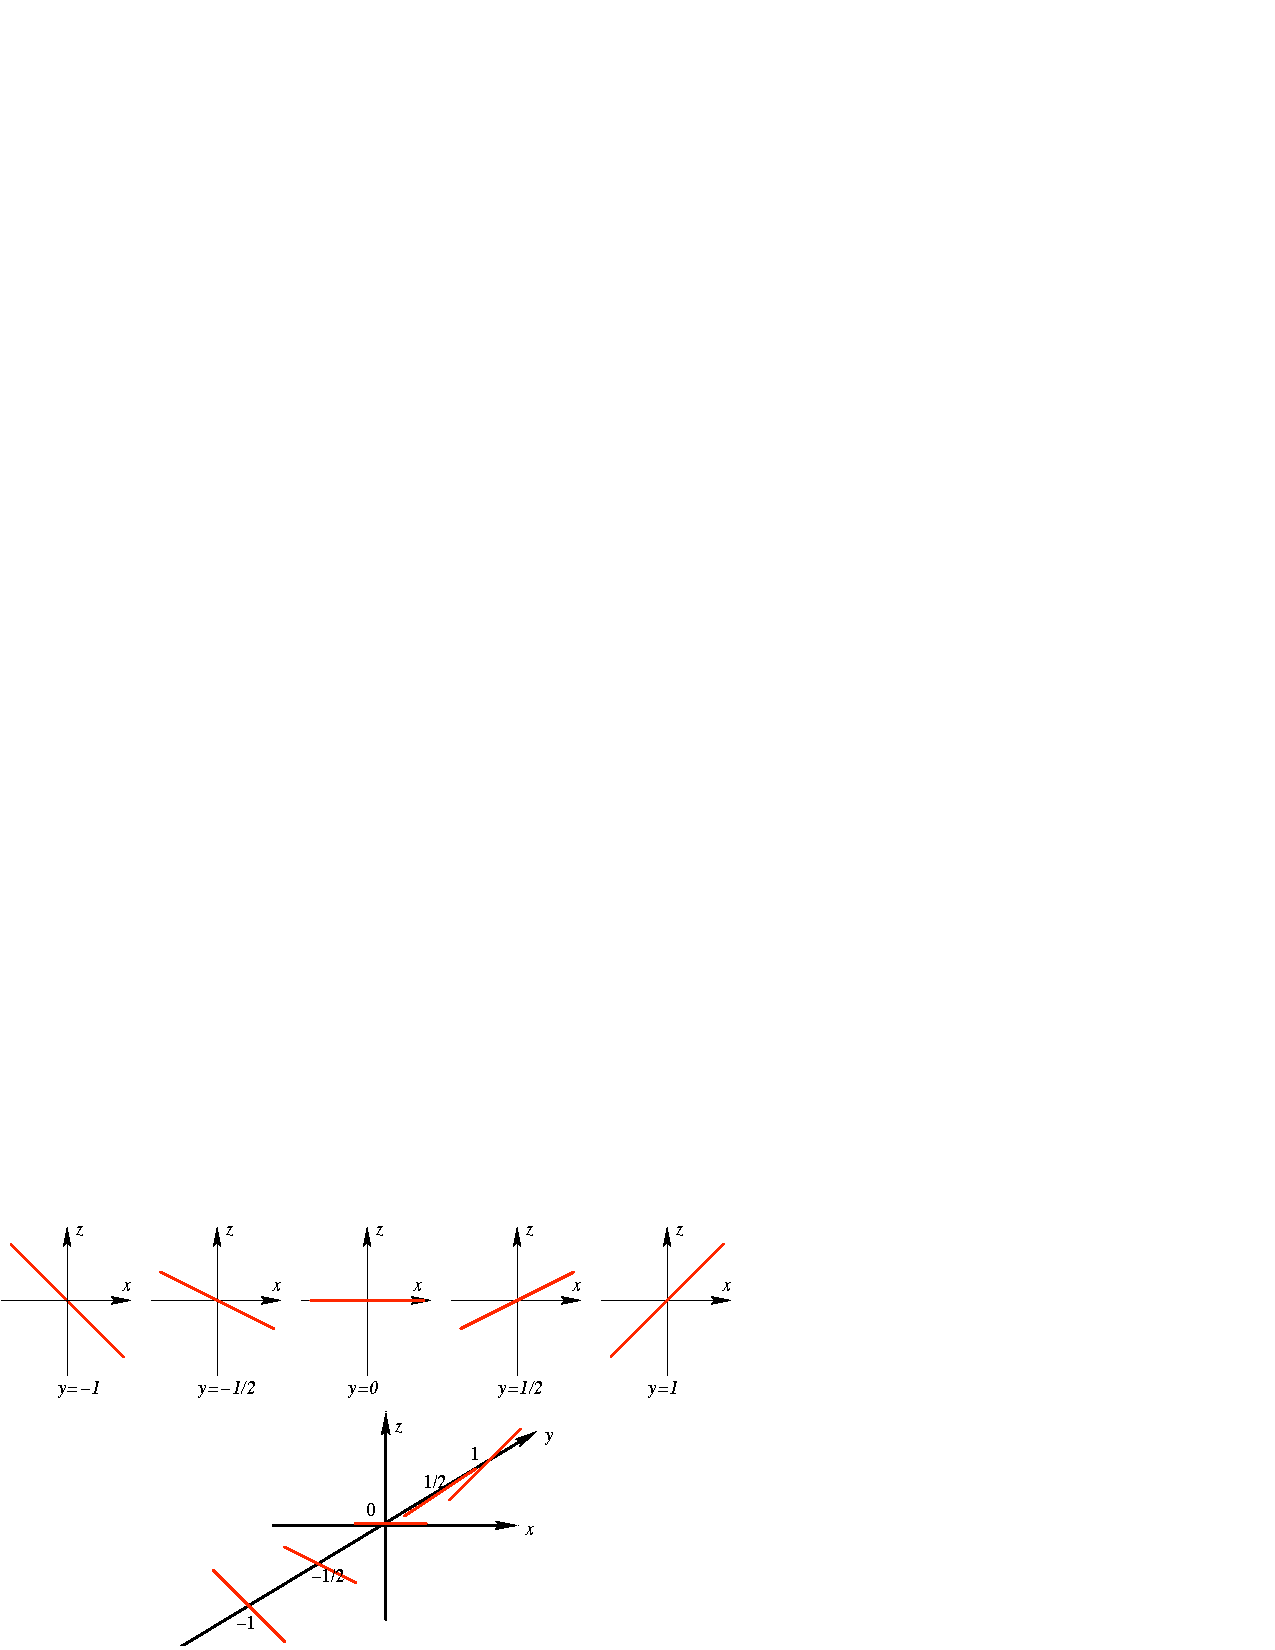
\includegraphics[scale=0.6]{01saddle1.pdf}}


The function $ z=xy $ is symmetric in the $ x $ and $ y $ variables,
so you get similar pictures if you freeze $ x $ and graph $ z=xy $ as
a function of $ y $.  Carefully putting both pictures together gives
something like this:

\centerline{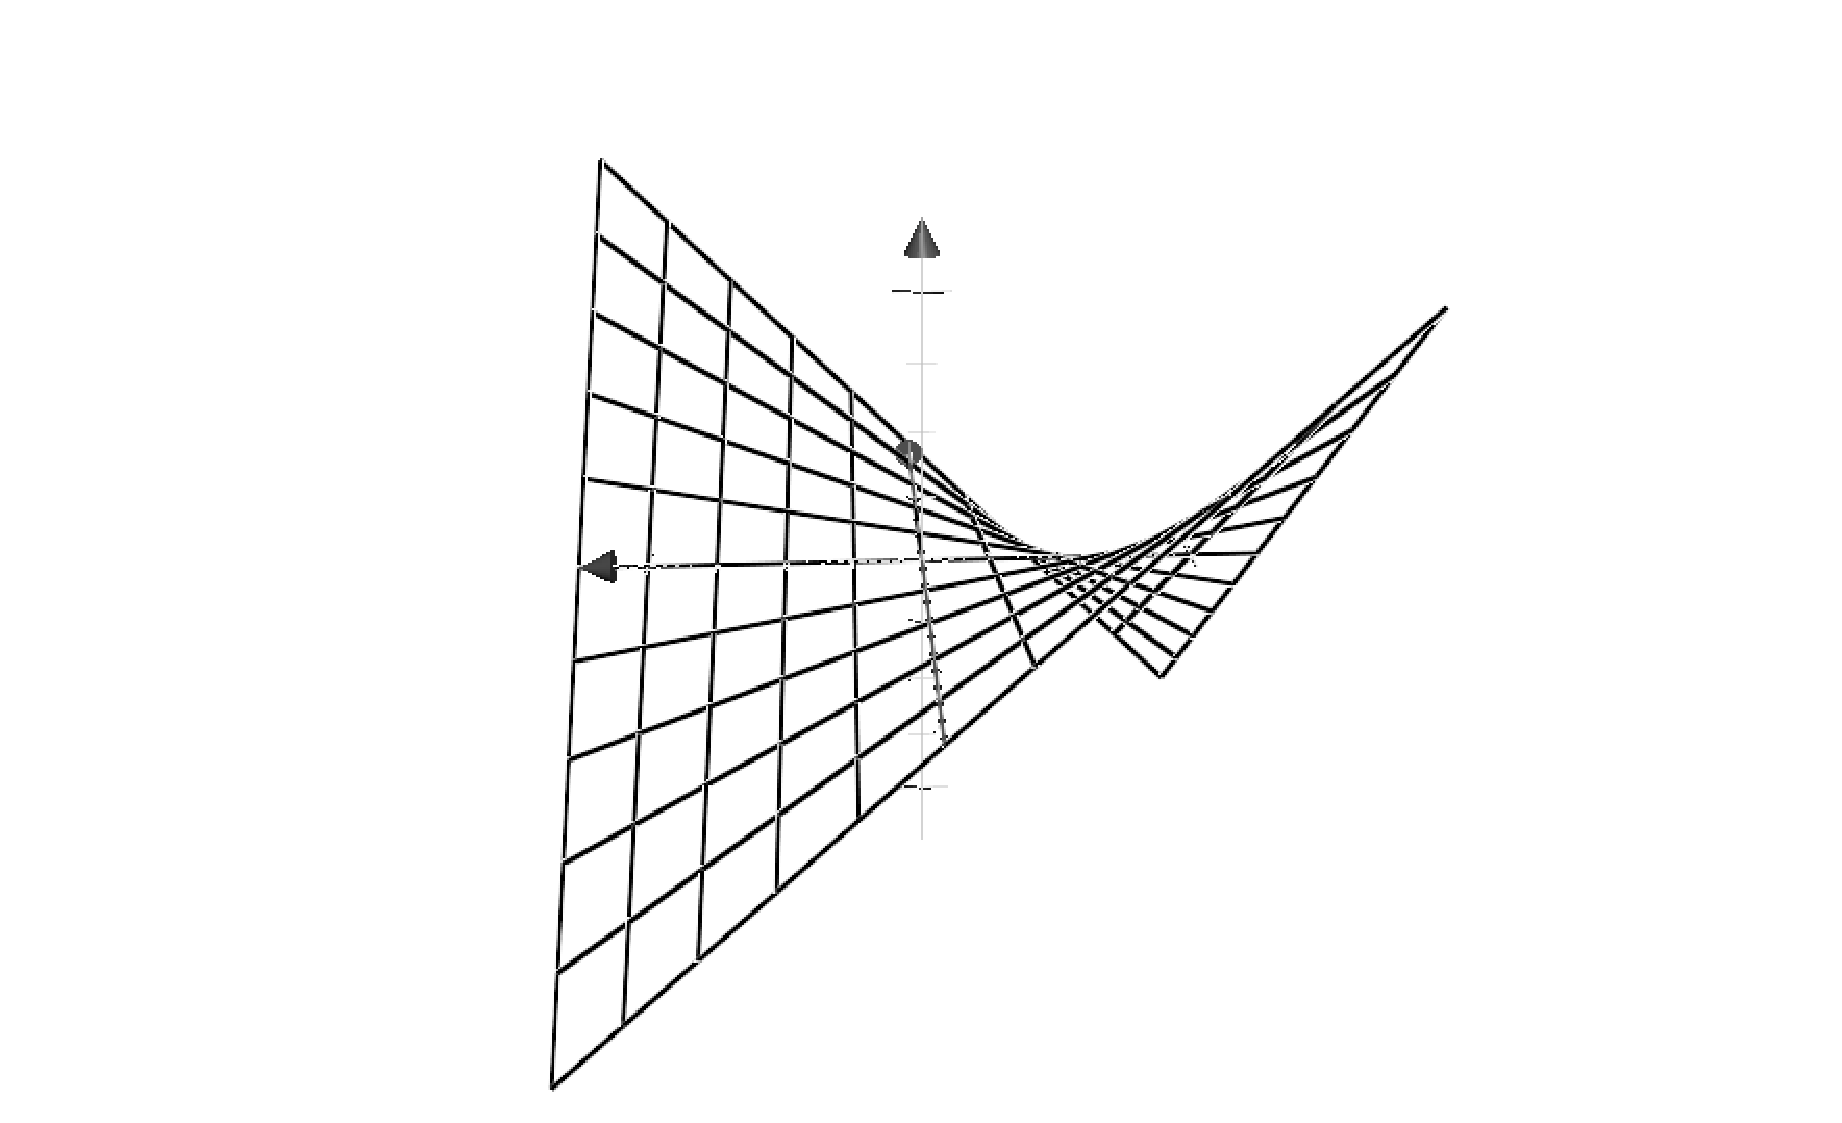
\includegraphics[width=0.3\textwidth]{01saddle3.pdf}}



\subsection{The domain of a function}    %{{{2

\begin{multicols}{2}

Just as with functions of one variable, functions of two variables
have a \emph{domain}, consisting of all the points $(x, y)$ in the
plain for which $f(x,y)$ is defined.  For functions of one variable
the domain is usually an interval, but for functions of two
variables the domain can have more interesting shapes.  In the
drawing on the left here, the function $f(x,y)$ is defined to be the
inverse of the distance from the point $(x, y)$ to the curve $E$ in
the picture.  This function is only defined when this distance is
not zero (otherwise you can't divide by the distance\ldots), so the
domain of this function consists of all points which do not lie on
the curve.

\centerline{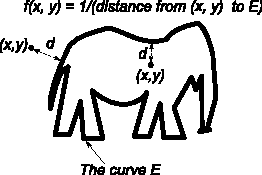
\includegraphics{01elephant.pdf}}
\end{multicols}
\subsection{Example}  What is the domain of the function     %{{{2
\[
f(x, y) = \frac{1}{\sqrt{1-x-y}}\quad??
\]
Clearly the function is defined if the quantity under the square root
is nonnegative (otherwise you can't take the square root), and not
zero (otherwise you can't divide by the resulting square root).  So
the domain consists of all points with $1-x-y>0$, or, equivalently,
$y<1-x$.  The domain consists of all points in the plane which line
below the graph of $y=1-x$.



\section{Open and closed sets in $\R^n$}    %{{{1
Intervals in the real line come in four kinds, depending on whether
they include their endpoints or not: you can have $(a,b)$, $(a, b]$,
$[a, b)$ and $[a,b]$, and those are all the possibilities.  With
domains in the plane, or in space there are many more possibilities,
and it will sometimes be important to distinguish between domains
which include all their ``endpoints'' and those that don't.  In the
present context one doesn't say ``endpoint'' but speaks of
\emph{boundary point} instead.  To define what a boundary point is, it
turns out that you need to resort to $\varepsilon$ and $\delta$ again,
or a least to $\varepsilon$.
Here is some terminology which we will use:
\begin{itemize}
\item $B_r(p)$ is the ball with center $p$ and radius $r$.

\item $G\subset \R^n$ is \emph{open} if for every point $p$ in $G$ there is an
  $\varepsilon>0$ such that $G$ contains $B_\varepsilon(p)$.

\item $G\subset\R^n$ is \emph{closed} if its complement is open.

\item $p$ is a \emph{boundary point} of $G$ if $B_r(p)$ always contains both
  points from $G$ and from its complement, no matter how small you
  choose $r>0$.
\end{itemize}
The following intuitive description is good enough for math 234: $G$
is closed if it contains all its boundary points; $G$ is open if it
contains none of its boundary points.

\begin{figure}[ht]\centering
  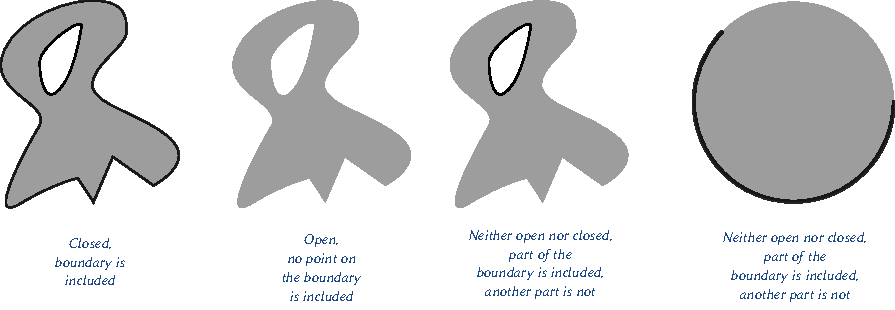
\includegraphics[width=\textwidth]{01openANDclosed.pdf}
  \caption{Some domains in the plane.  Points in the domain are shaded
  gray.  Boundary points which are included in the domain are marked
  in black.}
  \label{fig:01openANDclosed}
\end{figure}

\subsection{Example}\label{sec:openClosedExample} Consider the three domains    %{{{2
\begin{align*}
  G_1 &= \text{all points $(x, y)$ with $x^2+y^2<1$}\\
  G_2 &= \text{all points $(x, y)$ with $x^2+y^2\le1$}\\
  G_3 &= \text{all points $(x, y)$ with $-1\leq x\leq 1$ and
  $-\sqrt{1-x^2}<y\leq \sqrt{1-x^2}$}
\end{align*}
For all three domains the boundary points are the points on the unit
circle.  $G_1$ contains none of its boundary points, so it is called
``open'';  $G_2$ contains all its boundary points, so it is called
``closed'';  $G_3$ contains some but not all of its boundary points,
so it is neither open nor closed.



\section{More examples of visualization of Functions}    %{{{1

You can visualize a function $f$ of two variables by means of its
graph, but this is not the only way.  There are at least two
alternatives.  The first is in terms of \emph{level sets}, the other
is as a \emph{movie of a graph of a function of one variable}.

\emph{Level sets} are defined as follows.  Given a function $z=f(x,
y)$ and a number $c$, the level set at level $c$ is the set of all
points in the plane which satisfy $f(x, y) = c$; in symbols,
\[
\text{``Level set of $f$ at level $c$''} 
\stackrel{\rm def}{=}
\left\{ (x, y) : f(x, y) = c \right\}.
\]
To describe a function in terms of its level sets, one usually picks a
range of values for the constant $c$ and draws the level sets
corresponding to the chosen values of $c$ in one figure.

While the graph is a three-dimensional object, the level set is a set
of points in the plane, usually a curve.  Level sets are therefore
easier to draw than graphs.  

\subsection{Example}\label{sec:01levelsetexample}    %{{{2
What are the level sets of the function $f(x, y) = 3-x-y$?

For any given number $c$ the level set at level $c$ of $f$ contains
exactly those points $(x, y)$ which satisfy $f(x, y) = c$, i.e.\
$3-x-y = c$.  This is a line, and it is the graph of $y= 3-c-x$:  so
it is the line with slope $-1$ and ``$y$-intercept'' $3-c$.


\subsection{Level sets of the saddle surface}  What are the level sets    %{{{2
of the function whose graph we drew in \S~\ref{sec:example-of-a-function3}?

The function was given by $f(x, y)= xy$, so the level set at level
$c$ consists of all points $(x, y)$ in the plane which satisfy
$xy=c$.  For instance, if $c=1$, then you get the familiar hyperbola
$y=1/x$.  For other positive values of $c$ you get similar hyperbolas,
and for negative $c$ you get hyperbolas in the 2nd and 4th quadrants.

The level at $c=0$ is exceptional because it is not a hyperbola, but
rather consists of two crossing lines.  Namely, $xy=0$ holds when
either $x=0$ or $y=0$ holds, so the level set at $c=0$ is the union of
the $x$-axis and the $y$-axis.

\begin{figure}[htb]
  \begin{center}
    \begin{picture} (240.000000,176.533333)(0,0)
    \put(0.0, 0.0){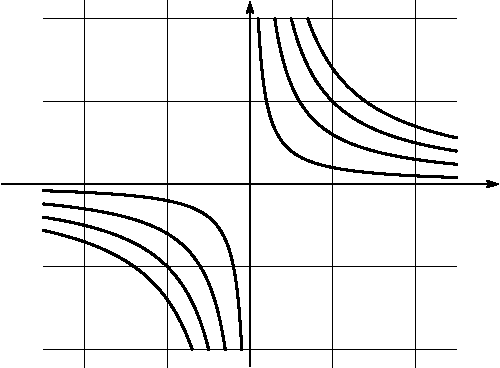
\includegraphics{01saddlelevels.pdf}}
        \put(221.17,  91.44){\sffamily\itshape \makebox[0pt][l]{{\footnotesize \tt$xy=$0.2}}}
    \put( 18.83,  83.09){\sffamily\itshape \makebox[0pt][r]{{\footnotesize \tt$xy=$0.2}}}
    \put(221.17,  97.79){\sffamily\itshape \makebox[0pt][l]{{\footnotesize \tt$xy=$0.6}}}
    \put( 18.83,  76.75){\sffamily\itshape \makebox[0pt][r]{{\footnotesize \tt$xy=$0.6}}}
    \put(221.17, 104.13){\sffamily\itshape \makebox[0pt][l]{{\footnotesize \tt$xy=$1.0}}}
    \put( 18.83,  70.40){\sffamily\itshape \makebox[0pt][r]{{\footnotesize \tt$xy=$1.0}}}
    \put(221.17, 110.48){\sffamily\itshape \makebox[0pt][l]{{\footnotesize \tt$xy=$1.4}}}
    \put( 18.83,  64.05){\sffamily\itshape \makebox[0pt][r]{{\footnotesize \tt$xy=$1.4}}}

\end{picture}

  \end{center}
  \caption{A few level sets of the function $f(x, y) = xy$.  Only
  positive levels are shown.  }
  \label{fig:saddlelevels}
\end{figure}


\subsection{An example from the ``real'' world}    %{{{2
\label{sec:01mendotaexample}  Here is a function of local interest.
The domain of the function is the water surface of Lake Mendota (let's
pretend this is a plane domain), and the function, which I'll call $d$
instead of $f$, is given by $d(x, y) = $ the depth of the lake at
location $(x, y)$.  There's no formula for this function, but the
limnology department of the UW has measured the depth and presented
the results in terms of the level sets of the function $d$.  


\begin{center}\sffamily
  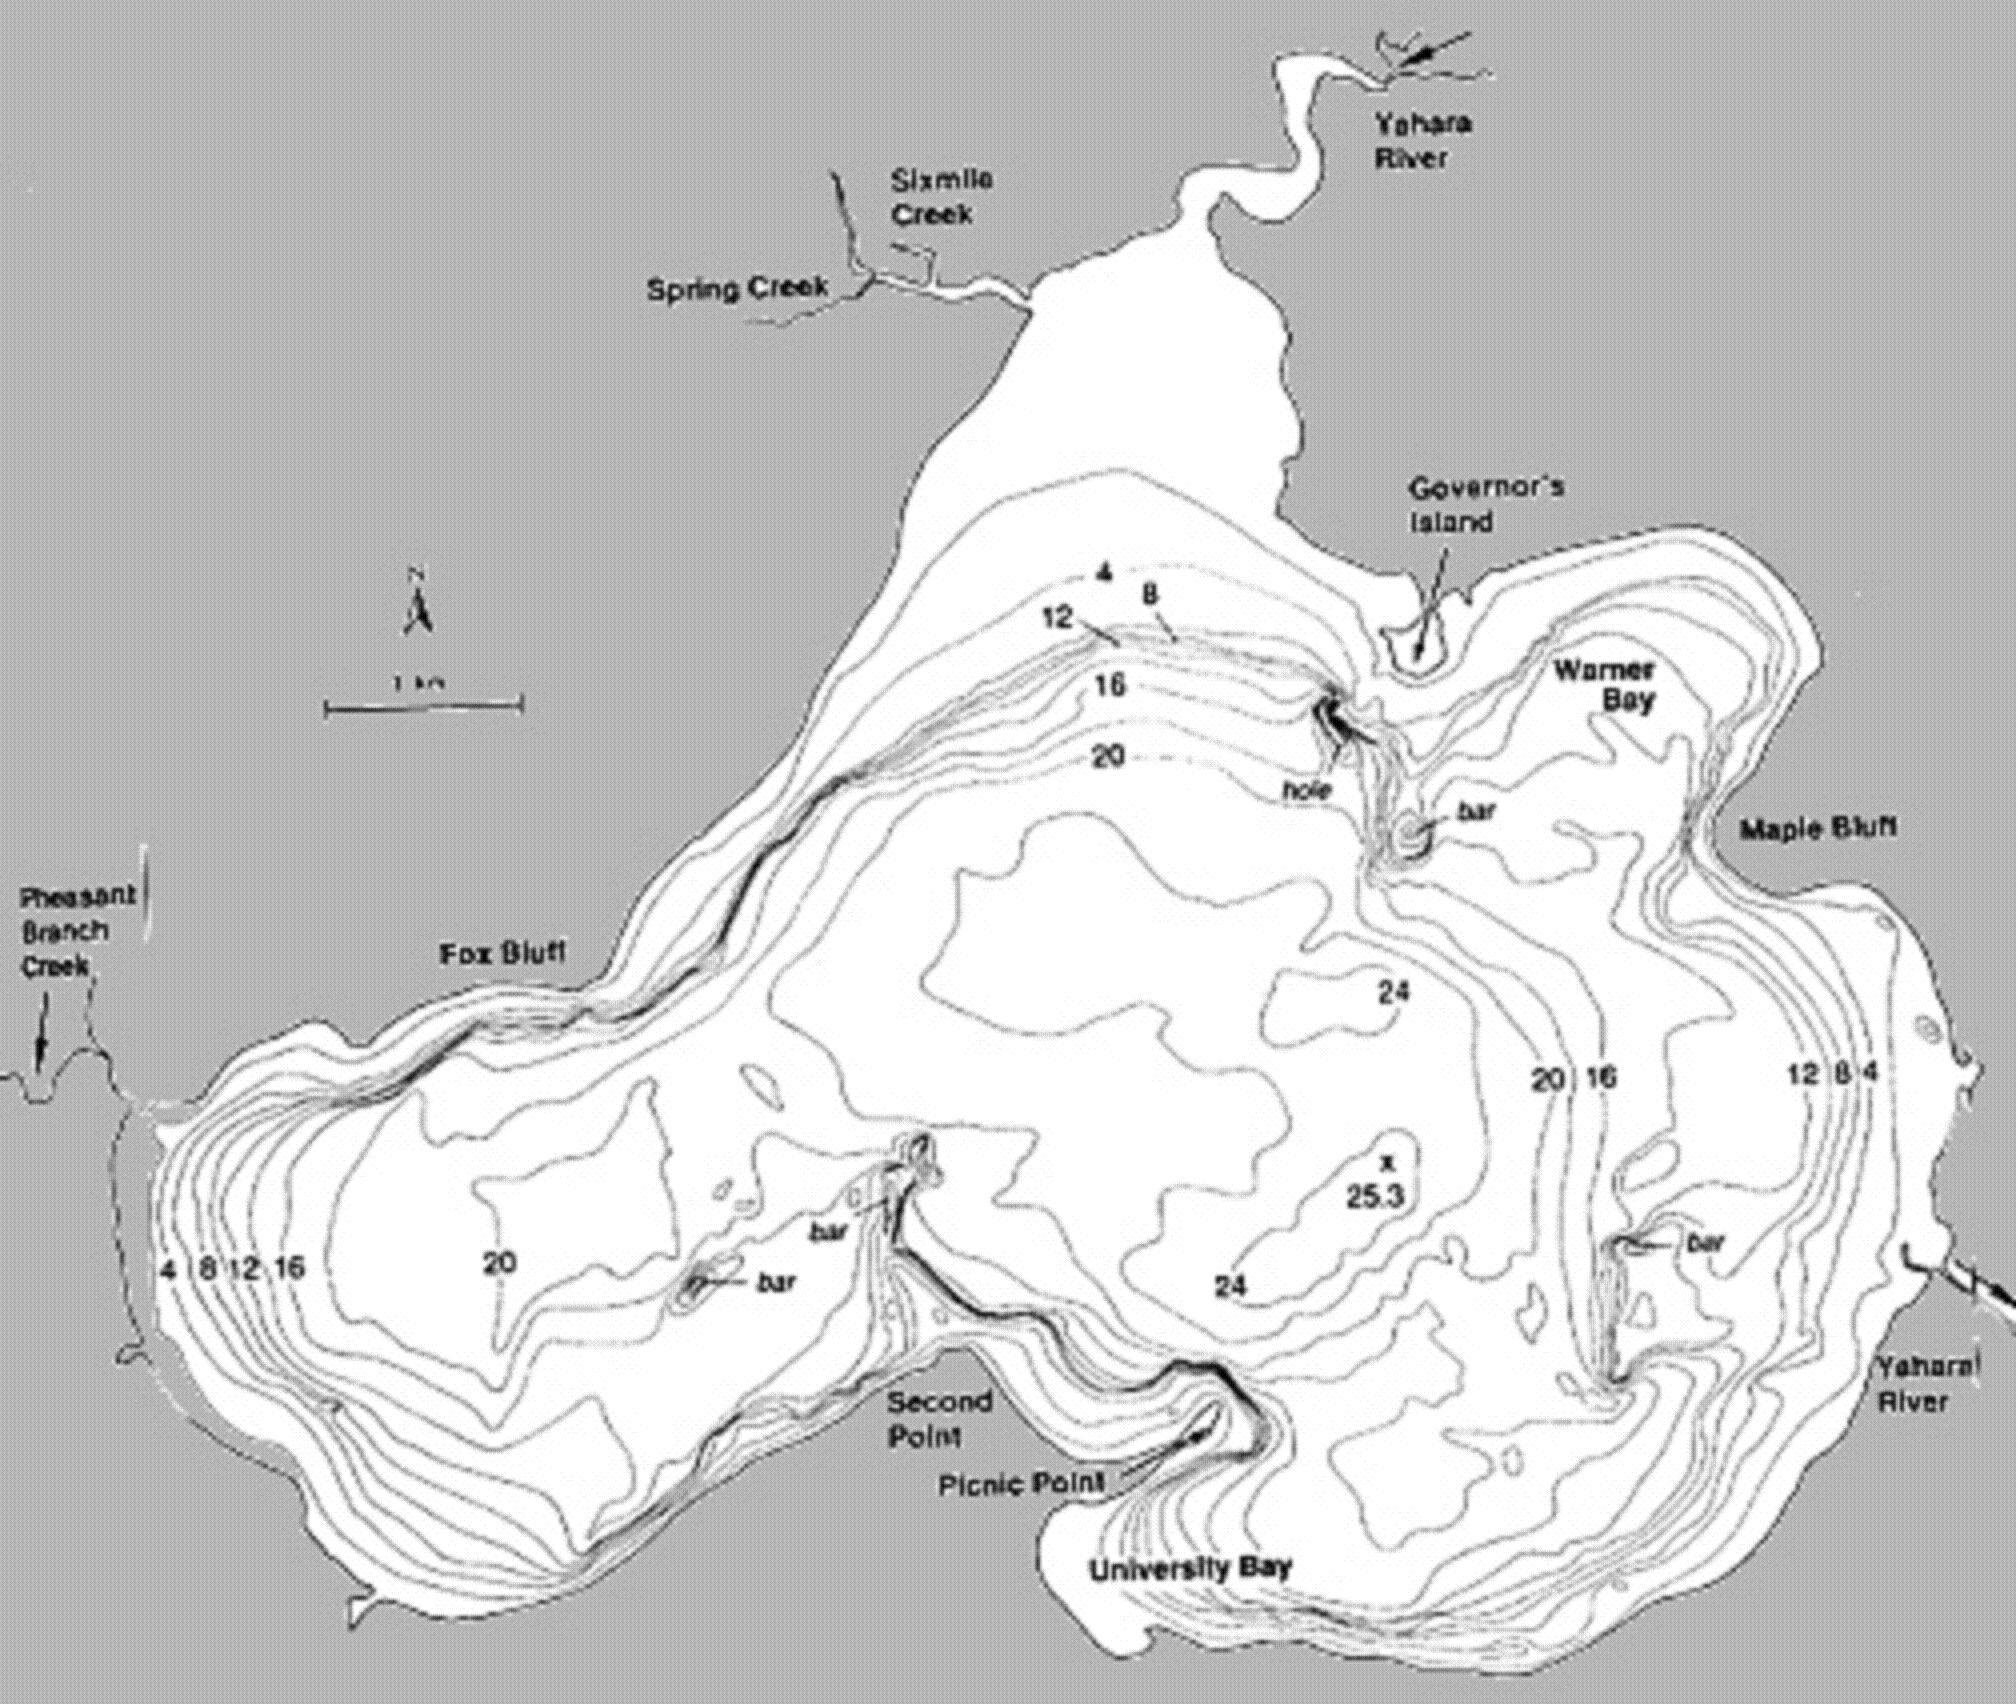
\includegraphics[width=0.75\textwidth]{01Mendota2.jpeg}
  
  The level curves of a function $z=d(x, y)$.  The domain
  of this function is the lake, \\
  and $d(x, y)$ is the depth in meters of Lake Mendota at $(x, y)$.\\
  See
  \url{http://limnology.wisc.edu/lake_information/mendota/mendota.html}
\end{center}


\subsection{Moving graphs}    %{{{2
There's another way of visualizing a function $z=f(x, y)$ of two
variables where you think of one of the independent variables (e.g.\
$y$) as ``time.''  The final picture is not one static picture of a
three dimensional surface, but rather a movie of a graph which is
moving around in the $xz$ plane.

If you have a function $z=f(x, y)$, then let us think of $y$ as time,
and let us relabel it as $t$, so that we are looking at the function
$z=f(x,t)$. Now at each moment in time $t$ we have a function $z=f(x,t)$
of one variable $x$ whose graph you can try to draw. Think of this graph
as a still-image. Then as you let time $t$ vary, putting the still images
in a sequence, you get a movie of a graph of a changing function of one
variable.

For instance, if the function is once again the saddle surface
function $z=xy$, then we would be considering the function $z=xt$. At
each moment $t$ the graph of $z=xt$ is a line with slope $t$. Putting
together these graphs gives a movie of a line which begins with a line
of rather negative slope;  during the movie the slope increases,
and in the middle our line has achieved horizontality;  finally, the
closing shot presents us with a line with a very positive slope.
Here are some stills from the movie:

\begin{center}
  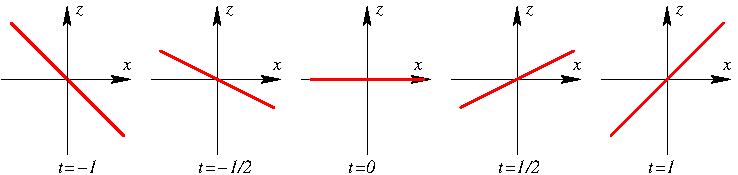
\includegraphics{01saddle-movie.pdf}
\end{center}

So you see that this interpretation is not very different from the
procedure of ``freezing the $y$ variable.'' The only real difference
lies in what you do with all the separate graphs you get after you
freeze a variable. In one case you try to piece them together to make a
bigger drawing of a three-dimensional object, in the other you put them
together to make a motion picture.



\section*{Problems}  %{{{1

\problemfont

In the problems in this stage of the course, you will be asked to
``sketch the graph of a function.''  From math 221 you remember that
this meant you had to find minima, maxima, inflection points, and other
features of the graph.  In 234 you will learn to do the same for
functions of two (and more) variables, but for now you should try to
use the method of ``freezing a variable'' or other similar tricks to
get an idea of what the graph of $f$ looks like.  

You can use a graphing program (such as \texttt{Grapher.app} on the
Mac, and \texttt{GraphCalc} on Windows) to check your answer.

\begin{center}
  \framebox{\parbox{0.4\textwidth}{Note: very often students try to
      fit their drawings into a region the size of a post-it.  In this
      course, whenever you make a drawing, especially if it's a
      three-dimensional drawing, \emph{make it large!}  Use half a
      page for a drawing.  Make sure you have enough paper, try to
      find lots of cheap scrap paper.}}
\end{center}

\problem  Make careful drawings of the graphs of the three functions
in the examples in \S\ref{sec:example-of-a-function1}, and
\S\ref{sec:example-of-a-function2}.


Find the domain of these functions.  Also, label the axes in every drawing
you make.

\problem\label{prb:some-functions}
Which functions of two variables $z=f(x, y)$ are defined by the
following formulae?  Find the domain of each function.  Then draw the
domain.  Try to sketch their graphs.  

\answer
\textbf{You should use a graphing program to produce pictures
of the graphs in these problems.}
\endanswer

\subprob $z-x^2=0$\hspace{7em}
\answer
$z-x^2=0$.
Domain $\R^2$.  Graph is a \emph{parabolic cylinder} and consists of
horizontal lines perpendicular to the $xz$-plane, going through the
parabola $y=x^2$ in that plane.

Level sets: parallel straight lines $x=\pm\sqrt{z}$ if $z>0$,
the $x$ axis if $z=0$, the empty set if $z<0$.
\endanswer
\subprob $z^2-x=0$\hspace{7em}
\answer
$z^2-x=0$.
Implicit function.
At least two functions are defined, namely $z=\pm \sqrt{x}$. 
Domain: all points $(x,y)$ with $x\ge 0$.
Graph is \emph{half a parabolic cylinder} and consists of
horizontal lines perpendicular to the $xz$-plane, going through the
parabola $z=\sqrt x$ (or $z=-\sqrt x$, depending on which function
you choose) in that plane.

Level sets (assuming we choose the function $z=+\sqrt{x}$):
the line $x=z^2$ if $z\ge0$, empty set otherwise.
\endanswer
\subprob $z-x^2-y^2=0$\\
\answer
$z-x^2-y^2=0$.
Domain is the whole plane.
Graph is a paraboloid of revolution, obtained by rotating the
parabola $z=x^2$ in the $xz$-plane around the $z$ axis.

Level sets: circle with radius $\sqrt{z}$ for $z>0$,
the origin for $z=0$ (note: this level set is a point rather than a curve),
empty for $z<0$.
\endanswer
\subprob $z^2-x^2-y^2=0$
\answer
$z^2-x^2-y^2=0$.
Implicit function.  Domain all of $\R^2$.
Possible functions are $z=\pm\sqrt{x^2+y^2}$.
Graph is the cone obtained by rotating the
half line $z=x, x\geq0$ in the $xz$-plane around the $z$ axis
(or the half line $z=-x, x\geq0$, if you chose $z=-\sqrt{x^2+y^2}$.)

Level sets (assuming we choose $z=+\sqrt{x^2+y^2}$):  circle with radius
$z$ when $z>0$, origin when $z=0$, empty when $z<0$.

\endanswer
\subprob $xyz=1$
\answer
$xyz=1$. 
Domain the whole plain with the $x$ and $y$-axes removed, i.e.\ all
points $(x, y)$ with $xy\ne0$.
Function is $f(x, y) = \frac{1} {xy}$.
For each $y$ the graph is the hyperbola $z=1/(yx)$ which is just the
standard hyperbola $z=1/x$ stretched vertically by a factor $1/y$.
As $y\to 0$ this factor goes to $\infty$.
\endanswer
\subprob $xy/z^2=1$\\
\answer
$xy/z^2=1$.
Implicit function.
Domain first and third quadrants (all points with $xy>0$).
Functions $z= \pm \sqrt{xy}$.
Cross sections with planes $y=$constant are half parabolas.

Note: Harder to see, but the surface with equation $xy=z^2$ is in fact
the cone obtained by rotating the $x$-axis around the line
$x=y$ in the $xy$-plane.
\endanswer
\subprob $x+y+z^2=0$
\subprob $x+y+z^2=1$

\problem Figure \ref{fig:saddlelevels} only presents level sets
$f(x, y)=c$ of the function $f(x, y) = xy$ for some \emph{positive} values
of $c$.  What does the zero set look like, and what do the level sets
$f(x, y) = c$ with $c<0$ look like?

\problem 
\label{prb:distance-to-square-level-sets}
Let $Q$ be the square in the plane consisting of all points $(x,y)$
with $|x|\le1$, $|y|\le1$.  This problem is about the so-called
\emph{distance function} to $Q$.  This function is defined as
follows:  $f(x, y)$ is the distance from the point $(x,y)$ to the
point in $Q$ nearest to $(x,y)$.

\subprob Which point in $Q$ is nearest to $(0, \frac12)$?  Which is
closest to $(0, 2)$?  Which is closest to $(3,4)$?
\answer
$(0, \frac{1} {2})$ is in the square $Q$, so it is the point closest to
$(0, \frac{1} {2})$.\\
The point $(0,1)$ on the top edge of the square is closest to $(0,2)$.\\
The corner point $(1,1)$ is closest to $(3,4)$.
\endanswer

\subprob Compute $f(0, \frac12)$, $f(0,2)$ and $f(3, 4))$.
\answer
$f(0, \frac12) =0 $;
$f(0,2)=1$ and $f(3, 4))=\sqrt{2^2+3^2}=\sqrt{13}$.
\endanswer

\subprob What is the zero set of $f$?
\answer
The zero set of $f$ is the square $Q$.
\endanswer

\subprob Draw the level sets of $f$ at levels $-1$, 1, 2, and 3.  Describe
the general level set $f(x, y) = c$ where $c$ is an arbitrary number.
\answer
The level set at level $-1$ is empty.  The others are ``rounded
rectangles,'' see this drawing, in which the square is grey, the dashed
lines are given by $x=\pm1$ or $y=\pm1$.
\begin{center}
    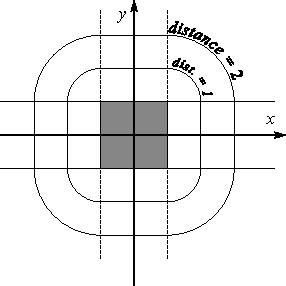
\includegraphics{01distancetosquare.pdf}
\end{center}
\endanswer

\subprob Give a formula for $f(x, y)$.  (It turns out too be hard to
capture the distance function in one formula.  You will have to split the
plane into different regions and describe $f(x,y)$ by different formulas,
according to which region $(x,y)$ belongs to.)
\answer
The lines $x=\pm1$ and $y=\pm1$ divide the plane into nine regions.
On each region the function is given by a different formula.
Here they are:
\begin{tabbing}
\=$\boldmath{f(x, y)}$ \=\`\textbf{ if } \ldots \\
\>$0$  \>\` $(x, y)$ in $Q$\\
\>$x-1$ \>\` $x\geq1, |y|\leq 1$\\
\>$y-1$ \>\` $|x|\leq 1, y\geq1$\\
\>$-x-1$ \>\` $x\le-1, |y|\leq 1$\\
\>$-y-1$ \>\` $|x|\leq 1, y\le-1$\\
\>$\sqrt{(x-1)^2+(y-1)^2}$ \>\` $x\ge1$ and $y\ge1$\\
\>$\sqrt{(x-1)^2+(y+1)^2}$ \>\` $x\ge1$ and $y\le-1$\\
\>$\sqrt{(x+1)^2+(y-1)^2}$ \>\` $x\le-1$ and $y\ge1$\\
\>$\sqrt{(x+1)^2+(y+1)^2}$ \>\` $x\le-1$ \& $y\le-1$\\
\end{tabbing}
\endanswer


\problem If $d(x, y)$ is the depth function of Lake Mendota (see
\S\ref{sec:01mendotaexample}), then what are the level sets $d(x, y) =
c$ for $c=0$, $c=+10$ and for $c=-10$ (meters)?  What is the level
set $d(x, y) = 400$ (meter)?

\problem For each of the functions in problem \ref{prb:some-functions}
draw the level sets at level $z=c$ for a few values of $c$ (as was
done in Figure \ref{fig:saddlelevels} and
\S~\ref{sec:01mendotaexample}).  What does the level set for an
arbitrary $c$ look like?  Are they familiar curves?
\answer
See answers to problem \ref{prb:some-functions}.
\endanswer

\problem Describe and explain the relation between the graph of the
function $y=g(x)$ of one variable, and the corresponding function
$f(x, y) = g\bigl( \sqrt{x^2+y^2} \bigr)$ of two variables.

What do the level sets of $f(x, y)$ look like?

For instance, if $g(x) = x$, then $f(x, y) = \sqrt{x^2+y^2}$: what is
the relation between the graphs of $g$ and $f$?
\answer
The graph of $f$ is obtained by taking the part of the graph of $z=g(x)$
with $x\ge0$ and rotating it around the $z$-axis.

Each level set of $f$ are circles, the origin, or is the empty set.


\endanswer


\problem Find the domain of the following functions of two (or occasionally
three) variables:

\subprob  $f(x, y) = \sqrt{9-x^2}+\sqrt{y^2-4}$\hspace{5em}
\answer
The two rectangular strips $-3\leq x\leq3, 2\leq y<\infty$ and
$-3\leq x\leq3, -\infty<y\leq-2$.
\endanswer

\subprob  $f(x, y) = \arcsin(x^2+y^2-2)$
\answer
By definition $\arcsin(x)$ is only defined if $-1\leq x\leq1$.
For $\arcsin(x^2+y^2-2)$ to be defined, we must therefore have
$-1\leq x^2+y^2-2 \leq 1$, i.e.\ $1\leq x^2+y^2 \leq 3$.

The domain of this function is 
the ring-shaped region between the circles with radii $1$ and
$\sqrt{3}$, both centered at the origin.
Circles are included in the domain.
\endanswer

\subprob  $f(x, y) = \sqrt{x}\;\cdot\;\sqrt{y}$
\answer
The way this function is written both $\sqrt x$ and $\sqrt y$ must be defined,
so the domain consists off all $(x,y)$ with $x\geq0$ and $y\geq0$. 
\endanswer

\subprob  $f(x, y) = \sqrt{xy}$
\answer
$\sqrt{xy}$ must exist, which happens for all $(x,y)$ in the first
and third quadrants (axes included.)
\endanswer

\subprob  $f(x, y, z) = 1/\sqrt{xyz}$

\subprob  $f(x, y) = \sqrt{16-x^2-4y^2}$
\answer
The region in the plane given by $x^2+4y^2\leq16$, which is the region
enclosed by an ellipse with
major axis of length 4, along the $x$ axis, and minor axis of length
2 along the $y$-axis.  The ellipse is included.
\endanswer

\problem\label{prb:cone-or-paraboloid}
Here are two sets of level curves with levels $z=0.2, 0.4, 0.6, 0.8,
1.0, 1.2,  1.4$.  One is for a function whose graph is a cone
($z=\sqrt{x^2+y^2}$), the other is for a paraboloid ($z=x^2+y^2$).
Which is which? Explain.

\begin{center}
  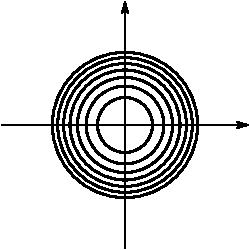
\includegraphics[scale=0.7]{01paraboloidLevels.pdf}
  \quad
  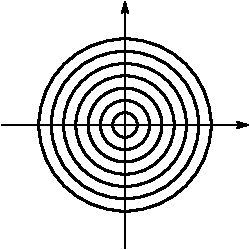
\includegraphics[scale=0.7]{01coneLevels.pdf}
\end{center}
\answer
The level sets of the function whose graph is a cone are equally spaced circles
(the level set at level $c$ is a circle with radius $c$).  Hence the one on the
right corresponds to the cone, and 
the one on the left corresponds to the paraboloid.
\endanswer


\section*{Problems about movies} %{{{1
\problem  Describe the ``movie'' that goes with each of the following
functions.

\subprob $f(x, t) = x\sin t$\hspace{6em}
\answer
At time $t$ we have a line through the origin with slope $\sin t$.
As time progresses this lines turns up and down, and up and down,  etc.
\endanswer
\subprob $f(x, t) = x\sin 2t$\hspace{6em}
\answer
Same as previous problem, but twice as fast.
\endanswer

\subprob $f(x, t) = t\sin x$
\answer
At all times one sees the graph of $y=\sin x$ stretched vertically by a factor $t$.
\endanswer

\subprob $f(x, t) = 2t \sin x$
\answer
Same as previous problem, but twice as fast.
\endanswer
\subprob $f(x, t) = t\sin 2x$
\answer
The graph of $y=\sin 2x$ stretched vertically by a factor $t$.
\endanswer

\subprob $f(x, t) = (x-t)^2$
\answer
Parabola with its minimum on the $x$-axis at $x=t$.
So we see the parabola $y=x^2$ translating from the left to the right
with constant speed 1.
\endanswer

\subprob $f(x, t) = (x-\sin t)^2$
\answer
Parabola with its minimum on the $x$-axis at $x=\sin t$.
So we see the parabola $y=x^2$ translating back and forth horizontally
every $2\pi$ time units.
\endanswer

\subprob $f(x, t) = (x-t^2)^2$

\subprob $f(x, t) = \dfrac{t^2}{1+x^2}$

\subprob $f(x, t) = \dfrac{1}{(1+x^2) (1+t^2)}$
\answer
At time $t$ we see Agnesi's witch, i.e. the graph $y= a/(1+x^2)$
with amplitude $a=1/(1+t^2)$.  Thus we see a bump whcich starts out small
 at $t=-\infty$, grows to its maximal size at time $t=0$, and then decays
again, until it vanishes at $t=+\infty$.
\endanswer


\problem
\label{prb:01traveling-waves} 
If $y=g(x)$ is any function of one variable, then a function of the
form $f(x, t) = g(x-ct)$ is often called a \emph{traveling wave} with
wave speed $c$ and profile $g$.  Let $g$ be any non constant
function of your choice and describe the movie presented by the
function $f(x, t) = g(x-ct)$ (can't choose?  Then try ``Agnesi's
witch'' $g(x) = \frac{1}{1+x^2}$.)

The number $c$ is called the wave speed.  If $c>0$ is the motion to
the left or to the right? Explain.
\answer
The graph of $y=g(x-a)$ is obtained from the graph of $y=g(x)$ by
translating the graph of $y=g(x)$ by $a$ units to the right.

Hence the graph of $g(x-ct)$ is the graph of $g(x)$ translated by $ct$
units to the right.  As time changes the graph of $g(x-ct)$ therefore
moves with velocity $c$ to the right.
\endanswer


\problem If $y=g(x)$ is any function of one variable, then a function
of the form $f(x, t) = \cos(\omega t) g(x)$ is often called a
\emph{standing wave.}
Let $g$ be any non constant function of your choice and describe the
movie presented by the function $f(x, t) = \cos(\omega t)g(x)$
(can't choose?  Then try ``Agnesi's witch''  $g(x) = \frac{1}{1+x^2}$
again, or for this example, try $g(x) = \sin x$.)

The number $\frac\omega{2\pi}$ is called the frequency of the standing
wave.  The function $g(x)$ is called its profile.  How long does it
take before the standing wave returns to its original position, i.e.\
what is the smallest $T>0$ for which $f(x, T) = f(x, 0)$ for all $x$?
Explain.

\answer
If you know the graph of a function $y=g(x)$, then you get
the graph of $y=cg(x)$ by stretching the graph of $g$ vertically by
a factor $c$ (here $c$ is a constant.)
If you allow this constant to depend on time, e.g.\ as in this
problem by setting $c=\cos(\omega t)$, then the ``movie'' you get is of a
version of the graph of $g$ which is growing and shrinking vertically.

\begin{center}
    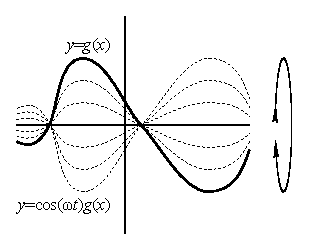
\includegraphics{01standingwave.pdf}
\end{center}
\endanswer


\section*{About open and closed sets} %{{{1

\problem Draw the sets $G_1, G_2, G_3$ from section
\ref{sec:openClosedExample} in the same style as
figure~\ref{fig:01openANDclosed} (i.e.\ shade the points in the region
and mark the boundary points which are included in the region).

\problem Using the intuitive description of when a set is open,
closed, or neither of those, discuss which of the intervals $(0,1)$,
$[0,1]$, $[0,1)$, and $(0,1]$ are open/closed/neither.

\problem (for discussion) Can you split the plane into two sets, both
of which are open?

\rmfamily\normalsize
%\end{multicols}

\section{Continuity and Limits}    %{{{1

\subsection{The limit of a function of two variables}    %{{{2
Just as with functions of one variable we need to define the limit of
$f(x, y)$ as $(x, y)$ approaches some given point $(a, b)$.  
There is again a precise definition involving epsilons and deltas, and
it is in many ways pretty much the same definition as in math 221.
Here it is:
\begin{definition}
  Let $f(x, y)$ be a function of two variables. Then we say that
  $$
  \lim_{(x, y) \to (a, b)} f(x, y) = L
  $$
  if for every $\varepsilon>0$ you can find a $\delta>0$ such that for
  all points $(x, y)$ one has
  \[
  \text{$(x, y)$ lies in $B_{\delta}(a, b)$} \implies
  |f(x, y) - L| <\varepsilon.
  \]
  \label{def:01limit}
\end{definition}

Remember that $B_\delta(a, b)$ is the disc with radius $\delta$ and
center $(a, b)$.  The last line of the definition therefore says that
you can be sure that $f(x, y)$ will be approximately equal to
$L$ with an error of no more than $\varepsilon$, provided you choose
$(x, y)$ so close to $(a,b)$ that the distance between $(x, y)$ and
$(a,b)$ is less than $\delta$.  The first part of the definition will
say that, no matter which $\varepsilon>0$ you come up with, a
$\delta>0$ can be found for which the second part is true.

In this course we will hardly ever use the above definition.  When we
have to compute limits we will use the limit properties, such as
\begin{gather}
  \lim_{(x, y) \to (a, b)} f(x, y) \pm g(x, y) =
  \Bigl\{\lim_{(x, y) \to (a, b)} f(x, y)\Bigr\}
  \pm
  \Bigl\{\lim_{(x, y) \to (a, b)} g(x, y)\Bigr\},
  \\
  \lim_{(x, y) \to (a, b)} f(x, y)g(x, y)
  =
  \Bigl\{\lim_{(x, y) \to (a, b)} f(x, y)\Bigr\}
  \quad\cdot\quad
  \Bigl\{\lim_{(x, y) \to (a, b)} g(x, y) \Bigr\}
  \\
  \lim_{(x, y) \to (a, b)} \frac{f(x, y)}{g(x, y)} =
  \frac{\DS
  \lim_{(x, y) \to (a, b)} f(x, y)}
  {\DS\lim_{(x,y)\to(a,b)} g(x, y)}
\end{gather}
where the latter holds only if $\lim_{(x, y) \to (a, b)} g(x, y) \neq
0$, and the interpretation of these formulas is that \emph{if} the
expression on the right exists, \emph{then} the limit on the left also
exists, and both are equal.

\begin{definition}[Definition of Continuity]
  \label{sec:def-of-continuity}
  A function $f(x, y)$ is called \emph{continuous} at a point
  $(a,b)$ in its domain if 
  \[
  \lim_{(x,y) \to (a,b)} f(x, y) = f(a,b).
  \]
\end{definition}

The precise meaning of continuity is expressed in terms of
$\varepsilon$'s and $\delta$'s, using definition \ref{def:01limit},
but the more important interpretation (for this course) of the
definition is that if $f$ is continuous at $(x=a, y=b)$, then the
function value $f(x, y)$ will be close to $f(a, b)$ if $x$ and
$y$ are both sufficiently close to $a$ and $b$, respectively.

In math 234 we do not study the techniques that can be used to prove
continuity of a function of two variables.  While there are many
discontinuous functions, most of these involve division by zero (see
examples below), or ``definition by parts'' (see problem
\ref{prb:stepfunction}), or more complicated constructions.

\begin{figure}[th]\centering
  \framebox{
  \begin{minipage}{0.49\textwidth}\sffamily\null 
    \begin{center}
      \bf Iterated Limits
    \end{center}
    Along path 1 you first send $x\to a$, and then $y\to b$, and this
    corresponds to the iterated limit
    \[
    \lim_{y\to b}\lim_{x\to a} f(x, y).
    \]
    If you first let $y\to b$ and then let $x\to a$, you get path 2,
    which corresponds to the other iterated integral.

    There are many other paths along
    which $(x, y)$ can approach $(a,b)$, and the limit
    \[
    \lim_{(x,y)\to (a,b)}f(x, y)
    \]
    equals some number $L$ if $f$ approaches this value no
    matter which path $(x, y)$ follows as it approaches $(a,b)$.
  \end{minipage}
  \begin{minipage}{0.49\textwidth}\sffamily
    \centering

    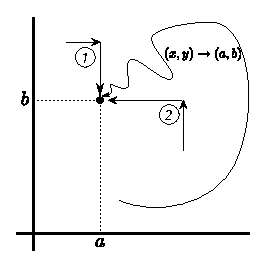
\includegraphics{01limitpaths.pdf}

  \end{minipage}

  }
\end{figure}

\subsection{Iterated limits} Instead of introducing a brand new    %{{{2
definition of ``limit'' you could try to recycle the old one-variable
definition of limit.  Thus, in order to find the limit of $f(x, y)$ as
$(x,y)$ approaches some point $(a,b)$, you could first forget about
$y$ and just let $x$ approach $a$.  This leads to
\[
\lim_{x\to a}f(x, y)  = L(y).
\]
This is a limit of one variable, because we're freezing the $y$
variable for the moment.  The result is some quantity which will
depend on the value at which we froze $y$.  Next you could let
$y$ approach $b$, and compute
\[
\lim_{y\to b} L(y) = \lim_{y\to b}\bigl\{\lim_{x\to a}f(x, y)\bigr\}.
\]
The result of this computation would then be our answer to the question
``what happens to $f(x, y)$ when $(x, y)$ goes to $(a, b)$?''

The problem here is that there are at least two versions of this
approach, depending on which limit you take first. You could compute
\[
\lim_{y\to b}\bigl\{\lim_{x\to a}f(x, y)\bigr\}
\text{ and }
\lim_{x\to a}\bigl\{\lim_{y\to b}f(x, y)\bigr\}.
\]
Do these always give the same result?  And do they give the same
result as the limit which we defined above in
\S\ref{sec:def-of-continuity}.  The answer to these questions is
``yes, most of the time, but not always.''

\subsection{Theorem on Switching Limits}\label{sec:01switching-limits}   %{{{2
\itshape \textbf{If} $\lim_{(x,y)\to (a, b)} f(x, y) = L$ exists,
\textbf{then} the two iterated limits exist, and they are the same:
\[
\lim_{x\to a}\lim_{y\to b} f(x,y) = \lim_{y\to b}\lim_{x\to a} f(x,y)
= L.
\]
Also, if $\lim_{(x,y)\to (a, b)} f(x, y) = L$ exists, and if $x(t)$
and $y(t)$ are any two functions with
\[
\lim_{t\to t_0} x(t) = a, \text{ and }
\lim_{t\to t_0} y(t) = b,
\]
(so that $(x(t),y(t))$ represents a path which approaches the point
$(a,b)$ as $t\to t_0$) then
\[
\lim_{t\to t_0}f(x(t), y(t)) = L.
\]

\upshape

\subsection{Limit examples}    %{{{2
\label{sec:limit-examples}
The function $f(x, y) = (x^2-y^2) / (x^2+y^2)$ is defined everywhere
on the plane, except at the origin.  You could try to assign a value
to $f(0,0)$ by taking the limit of $f(x,y)$ as $x$ and $y$ go to zero.
This is what you find :

Consider the limits
\[
A = \lim_{x\to 0}\lim_{y\to 0} \frac{x^2-y^2}{x^2+y^2} \text{ and }
B = \lim_{y\to 0}\lim_{x\to 0} \frac{x^2-y^2}{x^2+y^2}.
\]
Then you can easily compute that $A=1$ and $B=-1$.  So here is an
example where switching the order of limits changes the outcome.  
The theorem tells us that the limit
\[
\lim_{(x, y) \to (0,0)} \frac{x^2-y^2}{x^2+y^2}
\]
does not exist.

Note that to make this example we had to divide by zero at $(0,0)$.

\begin{figure}[ht]\centering
  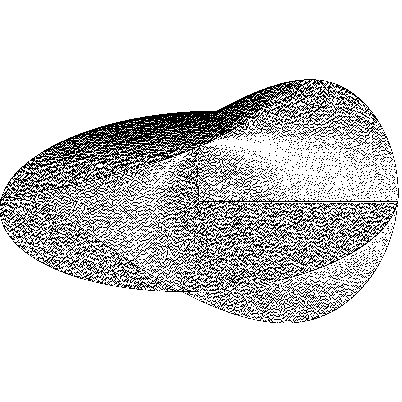
\includegraphics[scale=1.4]{01disco.pdf}
  \caption{The graph of a function which is discontinuous at the
  origin. (See Problem \ref {prb:01disco-axes}.)}
  \label{fig:01disco}
\end{figure}

Here is another example: consider the function
\[
g(x, y) = \frac{2xy}{x^2+y^2}.
\]
Its domain is the whole plane, except the origin, where we once again
would have to divide by zero.

The iterated limits exist for this example.  If you try to compute
them you will find
\[
\lim_{x\to 0}\lim_{y\to 0} \frac{2xy}{x^2+y^2} = 0, \text{ and }
\lim_{y\to 0}\lim_{x\to 0} \frac{2xy}{x^2+y^2} = 0 .  
\]
Nevertheless, the limit $\lim_{(x, y) \to (0,0)} g(x, y)$
\emph{does not exist}.  One way to see that is to let $(x, y)$
approach the origin along a straight line, say the line with equation
$y=x$. (What happens along other lines is one of the exercises).
You get
\[
\lim_{x\to 0, \; y=x} g(x, y) =
\lim_{x\to 0} g(x, x) = 
\lim_{x\to 0} \frac{2x\cdot x}{x^2+x^2} = 1.
\]
Conclusion: along the $x$-axis and along the $y$-axis $g$ remains 0, but
along the diagonal the function has the value $1$, so that its limit along
the diagonal is 1.



\section{Problems}   %{{{1

\begin{multicols}{2}\problemfont

\problem Find the level sets of the functions $f$ and $g$ from
\S\ref{sec:limit-examples}.
\answer
The level set at level $z=c$ is the set of points which satisfy
the equation
\[
\frac{x^2-y^2} {x^2+y^2} = c.
\]
You can simplify this equation by rewriting it as follows:
\begin{multline*}
  \frac{x^2-y^2} {x^2+y^2} = c \iff\\
  x^2-y^2 = cx^2+cy^2 \iff\\
  (1-c)x^2 = (1+c)y^2 \iff\\
  \frac{y} {x} = \pm\sqrt{\frac{1-c} {1+c}}.
\end{multline*}
So we see that if $\frac{1-c} {1+c}\geq0$ the level set
consists of two \emph{straight lines}, with the indicated slopes.
This happens exactly when $-1<c<1$.

When $c=\pm1$ we get either the equation $x^2=0$ or $y^2=0$, so
that the corresponding level sets consist of either the $y$-axis
or the $x$-axis.
\endanswer


\problem  Compute the limits of the functions $f$ and $g$ from
\S\ref{sec:limit-examples} along the lines $y=mx$, where $m$ is a
constant. Does the result depend on $m$?
\answer
For $f$ we have
\[
\lim_{x\to0}f(x, mx) = \lim_{x\to 0}\frac{x^2-m^2x^2} {x^2+m^2x^2}
=\frac{1-m^2} {1+m^2}.
\]
In fact this computation shows that $f$ is constant on lines
of the form $y=mx$, which we already found in the previous problem.
\endanswer


\problem
\label{prb:stepfunction}
Consider the function 
\[
f(x, y) = 
\begin{cases}
  1 & \text{if $y\geq |x|$} \\
  0 & \text{if $y<|x|$}.
\end{cases}
\]
\subprob Draw the graph of $f$.  What is its domain?
\answer
The function has been defined for all $(x,y)$, so
its domain is the whole plane.  The graph looks like this, roughly:

\begin{center}
    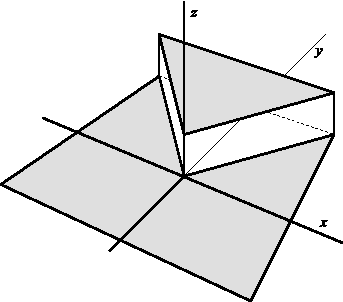
\includegraphics[width=120pt]{01jumpsonabs.pdf}
\end{center}

Note that the drawing doesn't tell you what the function values
are on the jump curve, $y=|x|$.
\endanswer


\subprob Compute the two iterated limits 
\[
A=\lim_{x\to0}\lim_{y\to0} f(x, y)
\]
and
\[
B=\lim_{y\to0}\lim_{x\to0} f(x, y).
\]
\answer
To compute $A$ we must take the limit as $x\to 0$ of $\lim_{y\to 0}f(x, y)$,
so we must know this limit when $x\neq 0$.

For all $x\neq0$ one has $\lim_{y\to 0}f(x, y) = 0$.
Hence $A = 0$.

To find $B$, compute for any $y\neq 0$
\[
\lim_{x\to0} f(x, y) =
\begin{cases}
  1 & \text{ if }y>0\\
  0 & \text{ if }y<0.
\end{cases}
\]
Hence the iterated limit
\[
\lim_{y\to0}\lim_{x\to0} f(x, y)
\]
does not exist (limits for $y\nearrow 0$ and $y\searrow 0$ are different).

\endanswer


\subprob Compute $\lim_{(x,y)\to(0,0)}f(x,y)$ if it exists.
\answer
The limit doesn't exist because one of the iterated limits $A$
and $B$ does not exist.
\endanswer



\subprob At which points $(a,b)$ in the plane is the function
continuous?
\answer
The function is continuous at all points $(x,y)$ except those with
$y=|x|$, where the function has a jump discontinuity.
\endanswer


\subprob Answer the same questions for the function
\[
g(x, y) = 
\begin{cases}
  1 & \text{if $|x|\leq y\leq 2|x|$} \\
  0 & \text{otherwise}.
\end{cases}
\]

\problem \label{prb:01disco-axes}
\subprob Figure \ref{fig:01disco} shows the
graph of
\[
f(x, y) = (x^2-y^2) / (x^2 + y^2)
\]
and the $xy$-plane (the plane $z=0	$).  The axes are missing.
Draw the $x$ and $y$ axes in the figure.

\subprob It turns out that the graph of
\[
g(x, y) = 2xy/(x^2+y^2)
\]
also looks like Figure~\ref{fig:01disco}.  Assuming that
Figure~\ref{fig:01disco} is in fact the graph of $g$, draw the
$x$ and $y$ axes in Figure~\ref{fig:01disco}.

\problem  Let
\[
h(x,y) = \frac{x^4-y^2}{x^4+y^2}.
\]

\subprob Compute the limit of $h(x, y)$ as $(x,y)$ approaches the
origin along the line $y=mx$.  Does the result depend on $m$?
\answer
\begin{align*}
  \lim_{\substack{(x, y)\to(0,0)\\y=mx}}& h(x,y)\\
  &=\lim_{x\to 0} h(x, mx)\\
  &=\lim_{x\to0} \frac{x^4 - m^2x^2} {x^4+m^2x^2}\\
  &=\lim_{x\to0} \frac{x^2 - m^2} {x^2+m^2}.
\end{align*}
If $m\neq0$ then this limit is
\[
\frac{-m^2} {m^2} = -1
\]
But when $m=0$ you get
\[
\lim_{x\to0} \frac{x^2 - m^2} {x^2+m^2}
=\lim_{x\to0} \frac{x^2} {x^2}
=1.
\]
\endanswer


\subprob Compute the limit of $h(x, y)$ as $(x,y)$ approaches the
origin along the parabola $y=mx^2$.  Does the result depend on $m$?
\answer
The two iterated limits
\[
\lim_{x\to0}\lim_{y\to0} h(x, y) = 1
\]
and
\[
\lim_{y\to0}\lim_{x\to0} h(x, y) = -1
\]
are different, so the limit $\lim_{(x,y)\to(0,0)}h(x, y)$ does not exist.
\endanswer


\subprob Does the limit $\lim_{(x,y)\to(0,0)}h(x, y)$ exist? 

\subprob Answer the same questions for the function
\[
k(x, y) = \frac{yx^2}{y^2+x^4}.
\]
\answer
\begin{align*}
  \lim_{\substack{(x, y)\to(0,0)\\y=mx^2}}& h(x,y)\\
  &=\lim_{x\to 0} h(x, mx^2)\\
  &=\lim_{x\to0} \frac{x^4 - m^2x^4} {x^4+m^2x^4}\\
  &=\lim_{x\to0} \frac{1 - m^2} {1+m^2}\\
  &=\frac{1 - m^2} {1+m^2}.
\end{align*}
So the answer does depend on $m$, i.e.\ depending
on which parabola $y=mx^2$ you follow to get to the origin,
you get a different limit.
\endanswer


\problem The following function plays an important role in the theory
of heat conduction, the theory of diffusion, and in probability
theory.  It is called the ``heat kernel'' or ``Gauss kernel''.
\[
H(x, t) = \frac{1}{\sqrt{t}} e^{-{x^2}/{t}}?
\]
Does the limit of $H(x, t)$ at $(0,0)$ exist?  Do any of the iterated
limits exist? More precisely,

\subprob Find $\DS \lim_{x\to 0}\lim_{t\searrow 0} H(x, t)$.

\subprob Find $\DS \lim_{t\searrow 0}\lim_{x\to 0} H(x, t)$.

(The domain of this function is all points $(x,t)$ with $t>0$ -- why?)

A hint:  How do you find the limit $\lim_{s\searrow
0}\frac{1}{\surd s}e^{-1/s}$?  You substitute $s=1/z$, so when $s\searrow 0$
you have $z\to+\infty$, and $\lim_{s\searrow 0}\frac1{\surd s} e^{-1/s} =
\lim_{z\to\infty} \sqrt z e^{-z}$.  Now use your math 221 limits.

\end{multicols}



%%% Local Variables: 
%%% mode: latex
%%% TeX-master: "free234"
%%% End: 
